
\documentclass[a4paper,12pt,openright]{book}
%\documentclass[a4paper, 12pt, openright, draft]{book}  Nalogo preverite tudi z opcijo draft, ki pokaže, katere vrstice so predolge! Pozor, v draft opciji, se slike ne pokažejo!
 
\usepackage[utf8]{inputenc}   % omogoča uporabo slovenskih črk kodiranih v formatu UTF-8
\usepackage[slovene,english]{babel}    % naloži, med drugim, slovenske delilne vzorce
\usepackage[pdftex]{graphicx}  % omogoča vlaganje slik različnih formatov
\usepackage{fancyhdr}          % poskrbi, na primer, za glave strani
\usepackage{amssymb}           % dodatni matematični simboli
\usepackage{amsmath}           % eqref, npr.
\usepackage{hyperxmp}
\usepackage[hyphens]{url}
\usepackage{csquotes}
\usepackage[pdftex, colorlinks=true,
						citecolor=black, filecolor=black, 
						linkcolor=black, urlcolor=black,
						pdfproducer={LaTeX}, pdfcreator={LaTeX}]{hyperref}

\usepackage{color}
\usepackage{soul}

\usepackage[
backend=biber,
style=numeric,
sorting=nty,
]{biblatex}


\addbibresource{literature.bib} %Imports bibliography file

\usepackage{listings} % For code showing

%%%%%%%%%%%%%%%%%%%%%%%%%%%%%%%%%%%%%%%%
%	DIPLOMA INFO
%%%%%%%%%%%%%%%%%%%%%%%%%%%%%%%%%%%%%%%%
% \newcommand{\fixspacing}{\vspace{0pt plus 1filll}\mbox{}}

\newcommand{\ttitle}{Pregled metod umetne inteligence v video igrah}
\newcommand{\ttitleEn}{Overview of Artificial Intelligence Approaches in Video Games}
\newcommand{\tsubject}{\ttitle}
\newcommand{\tsubjectEn}{\ttitleEn}
\newcommand{\tauthor}{Jovan Prodanov}
\newcommand{\tkeywords}{video igra, umetna inteligenca, pristopi, treniranje}
\newcommand{\tkeywordsEn}{video game, artificial intelligence, approaches, training}

\usepackage{hyperref}
%%%%%%%%%%%%%%%%%%%%%%%%%%%%%%%%%%%%%%%%
%	HYPERREF SETUP
%%%%%%%%%%%%%%%%%%%%%%%%%%%%%%%%%%%%%%%%
\hypersetup{pdftitle={\ttitle}}
\hypersetup{pdfsubject=\ttitleEn}
\hypersetup{pdfauthor={\tauthor, jp6957@student.uni-lj.si}}
\hypersetup{pdfkeywords=\tkeywordsEn}

%%%%%%%%%%%%%%%%%%%%%%%%%%%%%%%%%%%%%%%%
% PAGE SETUP
%%%%%%%%%%%%%%%%%%%%%%%%%%%%%%%%%%%%%%%% 
\addtolength{\marginparwidth}{-20pt} % robovi za tisk
\addtolength{\oddsidemargin}{40pt}
\addtolength{\evensidemargin}{-40pt}

\renewcommand{\baselinestretch}{1.3} % ustrezen razmik med vrsticami
\setlength{\headheight}{15pt}        % potreben prostor na vrhu
\renewcommand{\chaptermark}[1]
{\markboth{\MakeUppercase{\thechapter.\ #1}}{}} \renewcommand{\sectionmark}[1]
{\markright{\MakeUppercase{\thesection.\ #1}}} \renewcommand{\headrulewidth}{0.5pt} \renewcommand{\footrulewidth}{0pt}
\fancyhf{}
\fancyhead[LE,RO]{\sl \thepage} 
%\fancyhead[LO]{\sl \rightmark} \fancyhead[RE]{\sl \leftmark}
\fancyhead[RE]{\sc \tauthor}              % dodal Solina
\fancyhead[LO]{\sc Bachelor's thesis}     % dodal Solina

\newcommand{\BibTeX}{{\sc Bib}\TeX}

%%%%%%%%%%%%%%%%%%%%%%%%%%%%%%%%%%%%%%%%
% TITLES
%%%%%%%%%%%%%%%%%%%%%%%%%%%%%%%%%%%%%%%%  
\newcommand{\autfont}{\Large}
\newcommand{\titfont}{\LARGE\bf}
\newcommand{\clearemptydoublepage}{\newpage{\pagestyle{empty}\cleardoublepage}}
\setcounter{tocdepth}{1}	      % globina kazala

%%%%%%%%%%%%%%%%%%%%%%%%%%%%%%%%%%%%%%%%
% CONSTRUCTORS
%%%%%%%%%%%%%%%%%%%%%%%%%%%%%%%%%%%%%%%%  
% \newtheorem{izrek}{Izrek}[chapter]
% \newtheorem{trditev}{Trditev}[izrek]
% \newenvironment{dokaz}{\emph{Dokaz.}\ }{\hspace{\fill}{$\Box$}}

%%%%%%%%%%%%%%%%%%%%%%%%%%%%%%%%%%%%%%%%%%%%%%%%%%%%%%%%%%%%%%%%%%%%%%%%%%%%%%%
%% PDF-A
%%%%%%%%%%%%%%%%%%%%%%%%%%%%%%%%%%%%%%%%%%%%%%%%%%%%%%%%%%%%%%%%%%%%%%%%%%%%%%%

%%%%%%%%%%%%%%%%%%%%%%%%%%%%%%%%%%%%%%%% 
% define medatata
%%%%%%%%%%%%%%%%%%%%%%%%%%%%%%%%%%%%%%%% 
\def\Title{\ttitle}
\def\Author{\tauthor, jp6957@student.uni-lj.si}
\def\Subject{\ttitleEn}
\def\Keywords{\tkeywordsEn}

%%%%%%%%%%%%%%%%%%%%%%%%%%%%%%%%%%%%%%%% 
% \convertDate converts D:20080419103507+02'00' to 2008-04-19T10:35:07+02:00
%%%%%%%%%%%%%%%%%%%%%%%%%%%%%%%%%%%%%%%% 
\def\convertDate{%
    \getYear
}

{\catcode`\D=12
 \gdef\getYear D:#1#2#3#4{\edef\xYear{#1#2#3#4}\getMonth}
}
\def\getMonth#1#2{\edef\xMonth{#1#2}\getDay}
\def\getDay#1#2{\edef\xDay{#1#2}\getHour}
\def\getHour#1#2{\edef\xHour{#1#2}\getMin}
\def\getMin#1#2{\edef\xMin{#1#2}\getSec}
\def\getSec#1#2{\edef\xSec{#1#2}\getTZh}
\def\getTZh +#1#2{\edef\xTZh{#1#2}\getTZm}
\def\getTZm '#1#2'{%
    \edef\xTZm{#1#2}%
    \edef\convDate{\xYear-\xMonth-\xDay T\xHour:\xMin:\xSec+\xTZh:\xTZm}%
}

%\expandafter\convertDate\pdfcreationdate 

%%%%%%%%%%%%%%%%%%%%%%%%%%%%%%%%%%%%%%%%
% get pdftex version string
%%%%%%%%%%%%%%%%%%%%%%%%%%%%%%%%%%%%%%%% 
\newcount\countA
\countA=\pdftexversion
\advance \countA by -100
\def\pdftexVersionStr{pdfTeX-1.\the\countA.\pdftexrevision}


%%%%%%%%%%%%%%%%%%%%%%%%%%%%%%%%%%%%%%%%
% XMP data
%%%%%%%%%%%%%%%%%%%%%%%%%%%%%%%%%%%%%%%%  
\usepackage{xmpincl}
%\includexmp{pdfa-1b}

%%%%%%%%%%%%%%%%%%%%%%%%%%%%%%%%%%%%%%%%
% pdfInfo
%%%%%%%%%%%%%%%%%%%%%%%%%%%%%%%%%%%%%%%%  
\pdfinfo{%
    /Title    (\ttitle)
    /Author   (\tauthor, jp6957@student.uni-lj.si)
    /Subject  (\ttitleEn)
    /Keywords (\tkeywordsEn)
    /ModDate  (\pdfcreationdate)
    /Trapped  /False
}


%%%%%%%%%%%%%%%%%%%%%%%%%%%%%%%%%%%%%%%
% START
%%%%%%%%%%%%%%%%%%%%%%%%%%%%%%%%%%%%%%%
\begin{document}
\selectlanguage{english}
\frontmatter
\setcounter{page}{1} %
\renewcommand{\thepage}{}       % preprecimo težave s številkami strani v kazalu
\newcommand{\sn}[1]{"`#1"'}                    % dodal Solina (slovenski narekovaji)

%%%%%%%%%%%%%%%%%%%%%%%%%%%%%%%%%%%%%%%%
% INTRO
%%%%%%%%%%%%%%%%%%%%%%%%%%%%%%%%%%%%%%%%
 \thispagestyle{empty}%
   \begin{center}
    {\large\sc Univerza v Ljubljani\\%
      Fakulteta za računalništvo in informatiko}%
    \vskip 10em%
    {\autfont \tauthor\par}%
    {\titfont \ttitle \par}%
    {\vskip 2em \textsc{DIPLOMSKO DELO\\[2mm]
    VISOKOŠOLSKI STROKOVNI ŠTUDIJSKI PROGRAM PRVE STOPNJE RAČUNALNIŠTVO IN INFORMATIKA}\par}%
    \vfill\null%
    {\large \textsc{Mentor}: doc.\ dr.  Aleš Jaklič\par}%
    {\vskip 2em \large Ljubljana, 2022 \par}%
\end{center}

\clearemptydoublepage

%%%%%%%%%%%%%%%%%%%%%%%%%%%%%%%%%%%%%%%%
% INTRO ENGLISH
%%%%%%%%%%%%%%%%%%%%%%%%%%%%%%%%%%%%%%%%
 \thispagestyle{empty}%
   \begin{center}
    {\large\sc University of Ljubljana\\%
      Faculty of Computer and Information Science}%
    \vskip 10em%
    {\autfont \tauthor\par}%
    {\titfont \ttitleEn \par}%
    {\vskip 2em \textsc{Bachelor's Thesis\\[2mm]
    PROFESSIONAL STUDY PROGRAM UNDERGRADUATE PROGRAMMES COMPUTER AND INFORMATION SCIENCE}\par}%
    % Not sure if correct "University"
    \vfill\null%
    {\large \textsc{Mentor}: doc.\ dr.  Aleš Jaklič\par}%
    {\vskip 2em \large Ljubljana, 2022 \par}%
\end{center}


\newcommand{\CcImageCc}[1]{%
	
\includegraphics[scale=#1]{cc_cc_30.pdf}%
}
\newcommand{\CcImageBy}[1]{%
	
\includegraphics[scale=#1]{cc_by_30.pdf}%
}
\newcommand{\CcImageSa}[1]{%
	
\includegraphics[scale=#1]{cc_sa_30.pdf}%
}

%%%%%%%%%%%%%%%%%%%%%%%%%%%%%%%%%%%%%%%%
% copyright page
%%%%%%%%%%%%%%%%%%%%%%%%%%%%%%%%%%%%%%%%
\newpage
\thispagestyle{empty}

\vspace*{5cm}
{\small \noindent
To delo je ponujeno pod licenco \textit{Creative Commons Priznanje avtorstva-Deljenje pod enakimi pogoji 2.5 Slovenija} (ali novej\v so razli\v cico).
To pomeni, da se tako besedilo, slike, grafi in druge sestavine dela kot tudi rezultati diplomskega dela lahko prosto distribuirajo,
reproducirajo, uporabljajo, priobčujejo javnosti in predelujejo, pod pogojem, da se jasno in vidno navede avtorja in naslov tega
dela in da se v primeru spremembe, preoblikovanja ali uporabe tega dela v svojem delu, lahko distribuira predelava le pod
licenco, ki je enaka tej.
Podrobnosti licence so dostopne na spletni strani \href{http://creativecommons.si}{creativecommons.si} ali na Inštitutu za
intelektualno lastnino, Streliška 1, 1000 Ljubljana.

\vspace*{1cm}
\begin{center}% 0.66 / 0.89 = 0.741573033707865
\CcImageCc{0.741573033707865}\hspace*{1ex}\CcImageBy{1}\hspace*{1ex}\CcImageSa{1}%
\end{center}
}

\vspace*{1cm}
{\small \noindent
Izvorna koda diplomskega dela, njeni rezultati in v ta namen razvita programska oprema je ponujena pod licenco GNU General Public License,
različica 3 (ali novejša). To pomeni, da se lahko prosto distribuira in/ali predeluje pod njenimi pogoji.
Podrobnosti licence so dostopne na spletni strani \url{http://www.gnu.org/licenses/}.
}

\vfill
\begin{center} 
\ \\ \vfill
{\em
Besedilo je oblikovano z urejevalnikom besedil \LaTeX.}
\end{center}

% prazna stran
\clearemptydoublepage

%%%%%%%%%%%%%%%%%%%%%%%%%%%%%%%%%%%%%%%%
% stran 3 med uvodnimi listi
\thispagestyle{empty}
\
\vfill

\bigskip
\noindent\textbf{Kandidat:} \tauthor\\
\noindent\textbf{Naslov:} \ttitle\\
\noindent\textbf{Vrsta naloge:} Diplomska naloga na visokošolskem programu prve stopnje Računalništvo in informatika \\
\noindent\textbf{Mentor:} doc. dr. Aleš Jaklič\\

\bigskip
\noindent\textbf{Opis:}\\
Izdelajte pregled najpogostejših metod umetne inteligence v video igrah. Podrobneje preučite možnosti uporabe v razvojnem okolju Unity. Rabo pristopov ilustrirajte s preprostimi primeri v okolju Unity.

\bigskip
\noindent\textbf{Title:} \ttitleEn

\bigskip
\noindent\textbf{Description:}\\
Write an overview of the most common artificial intelligence approaches in video games. Provide a study of possible uses in Unity development environment. Illustrate the methods with simple examples in Unity environment.

\vfill

\vspace{2cm}

% prazna stran
\clearemptydoublepage

% zahvala
\thispagestyle{empty}\mbox{}\vfill\null\it%
\noindent
Zelo sem hvaležen vsem, ki so mi pomagali priti tja, kjer sem.
\rm\normalfont

% prazna stran
\clearemptydoublepage

%%%%%%%%%%%%%%%%%%%%%%%%%%%%%%%%%%%%%%%%
% posvetilo, če sama zahvala ne zadošča :-)
%%%%%%%%%%%%%%%%%%%%%%%%%%%%%%%%%%%%%%%%

% \thispagestyle{empty}\mbox{}{\vskip0.20\textheight}\mbox{}\hfill\begin{minipage}{0.55\textwidth}%
% Za svoja draga družina.
% \normalfont\end{minipage}

% % prazna stran
% \clearemptydoublepage


%%%%%%%%%%%%%%%%%%%%%%%%%%%%%%%%%%%%%%%%
% kazalo
\pagestyle{empty}
\def\thepage{}% preprecimo tezave s stevilkami strani v kazalu
\tableofcontents{}


% prazna stran
\clearemptydoublepage


%%%%%%%%%%%%%%%%%%%%%%%%%%%%%%%%%%%%%%%%
% List of abbriviations
%%%%%%%%%%%%%%%%%%%%%%%%%%%%%%%%%%%%%%%%

% \chapter*{Seznam uporabljenih kratic}  % spremenil Solina, da predolge vrstice ne gredo preko desnega roba
\chapter*{List of abbreviations used}  % spremenil Solina, da predolge vrstice ne gredo preko desnega roba

\noindent\begin{tabular}{p{0.21\textwidth}|p{.4\textwidth}|p{.4\textwidth}}    % po potrebi razširi prvo kolono tabele na račun drugih dveh!
    % {\bf kratica} & {\bf angleško} & {\bf slovensko} \\ \hline
  {\bf Abbreviation} & {\bf English} & {\bf Slovenian} \\ \hline
  % after \\: \hline or \cline{col1-col2} \cline{col3-col4} ...
  {\bf AI}      & artificial intelligence           & umetna inteligenca \\
  {\bf ML}      & machine learning                  & strojno učenje \\
  {\bf FSM}     & finite state machine              & končni avtomat \\
  {\bf NN}      & neural network                    & nevronska mreža \\
  {\bf NPC}     & non-player character              & neigralski lik \\
  {\bf BT }     & behaviour trees                   & drevesa vedenja \\
  {\bf RL }     & reinforcement learning            & spodbujevano učenje \\
  {\bf API }    & Application Programming Interface & aplikacijski programski vmesnik \\
  \dots         & \dots                             & \dots \\
\end{tabular}

% prazna stran
\clearemptydoublepage

%%%%%%%%%%%%%%%%%%%%%%%%%%%%%%%%%%%%%%%%
% povzetek
%%%%%%%%%%%%%%%%%%%%%%%%%%%%%%%%%%%%%%%%

\addcontentsline{toc}{chapter}{Povzetek}
\chapter*{Povzetek}

\noindent\textbf{Naslov:} \ttitle
\bigskip

\noindent\textbf{Avtor:} \tauthor
\bigskip

%\noindent\textbf{Povzetek:} 
\noindent 
V diplomski nalogi bodo predstavljeni različni načini uporabe umetne inteligence v računalniških igrah s poudarkom na orodju, ki uporablja globoko spodbujevano učenje. Poglobili se bomo v zajčjo luknjo, ki je umetna inteligenca iger in poskušali razumeti leta raziskav. Celotne zgodovine umetne inteligence iger ne bomo zajeli, vendar bo dovolj da ugotovimo kaj pomeni.
\bigskip

\noindent\textbf{Ključne besede:} \tkeywords.
% prazna stran
\clearemptydoublepage


%%%%%%%%%%%%%%%%%%%%%%%%%%%%%%%%%%%%%%%%
% abstract
%%%%%%%%%%%%%%%%%%%%%%%%%%%%%%%%%%%%%%%%

\selectlanguage{english}
\addcontentsline{toc}{chapter}{Abstract}
\chapter*{Abstract}

\noindent\textbf{Title:} \ttitleEn
\bigskip

\noindent\textbf{Author:} \tauthor
\bigskip

%\noindent\textbf{Abstract:} 
\noindent 
The thesis will present different ways of using artificial intelligence in computer games with an emphasis on a tool that uses deep reinforcement learning.
We will go deep into the rabbit hole that is game AI and try to understand years of research. The whole history of game AI will not be covered, but it will be enough to figure out what it means.
\bigskip



\noindent\textbf{Keywords:} \tkeywordsEn.
\selectlanguage{english}
% prazna stran
\clearemptydoublepage


% Daljsi povzetek

\addcontentsline{toc}{chapter}{Daljši povzetek}
\chapter*{Daljši povzetek}

\noindent\textbf{Naslov:} \ttitle
\bigskip

\noindent\textbf{Avtor:} \tauthor
\bigskip

Ko so bile video igre ustvarjene, so ljudje razmišljali o številnih načinih, kako bi jih naredili bolj zanimive. Eden od teh načinov je bilo ustvarjanje posebnega zabavnega vedenja v njih. To vedenje je lahko karkoli v igri, ta diplomska naloga pa se bolj osredotoča na vedenje likov, ki uporabljajo nekakšno umetno inteligenco.

Problem umetne inteligence v igrah je uporaba različnih pristopov, katere bom v tej diplomski nalogi poskušal predstaviti. Umetna inteligenca je nepredvidljiva in se vedno uči, zato je v nasprotju s tem, kar bi morale biti video igre. Nasprotniki ali liki v video igrah so narejeni za zabavo in izziv igralca na določeno raven. Če igralec dobi umetno izboljšanega nasprotnika in ga premaga na vseh ravneh, bi se hitro začeli dolgočasiti in bi bilo nemogoče igrati.

Tako so se skozi leta razvijalci iger trudili in ustvarili napredne tehnike za vse vrste vedenja, da bi bilo igranje video iger zabavno. Ta diplomska naloga bo obravnavala nekaj od številnih tehnik umetne inteligence na način, da bomo spoznali, kako delujejo na zabaven in učinkovit način. Prav tako so za nekaj izmed njih izdelani primeri, ki kažejo moč določene tehnike umetne inteligence v igri. Pristopi so sestavljeni iz številnih že videnih, a na koncu je ena eksperimentalna tehnologija, ki mi je bila zelo všeč. Pristopi so:

\clearpage


\begin{enumerate}
    \item Finite state machines
        \begin{itemize}
            \item Pokazali so, da so zelo uporabni v igrah, saj uporabljajo stanja in prehode z veliko razširljivosti. Vendar so za igre, ki imajo vnaprej dober načrt, saj so zelo omejene in za bolj poglobljeno karakterizacijo igre bi bilo potrebno nekaj bolj prilagodljivega.
        \end{itemize}
    \item Behaviour/Decision Trees
        \begin{itemize}
            \item Sestavljeni so iz vozlišč, ki so vedenja, in pogojev za vsako vozlišče. So zelo učinkoviti v video igrah, vendar se je pokazalo, da zahtevajo veliko računske moči.
        \end{itemize}
    \item Scripting
        \begin{itemize}
            \item Gre za kontroverzno temo, saj so najboljše in najslabše igre nastale iz skriptiranja. Z dobrim načrtom in v kombinaciji z drugo tehnologijo umetne inteligence lahko privede do zelo dobrih rezultatov.
        \end{itemize}
    \item Fuzzy logic
        \begin{itemize}
            \item To je logika, ki lahko vsebuje spremenljivke delne resnice, zato jo je mogoče učinkovito uporabiti v video igrah.
        \end{itemize}
    \item Flocking
        \begin{itemize}
            \item Je način za simulacijo gibanja čred v videoigri, uporablja nekaj algoritmov za iskanje poti in je zelo učinkovit v strateških igrah.
        \end{itemize}
    \item Genetics algorithm
        \begin{itemize}
            \item Gre po načelih Darwinove teorije, z mutiranjem in razmnoževanjem generacij dobimo zelo dobre rezultate za umetno inteligenco.
        \end{itemize}
        \clearpage
    \item Package ML-Agents
        \begin{itemize}
            \item Orodje, ki uporablja spodbujevano učenje za usposabljanje agentov, s tem pa ustvari "možgane", ki jih je mogoče uporabiti v likih video igric.
        \end{itemize}
\end{enumerate}

Ko dojamemo različne pristope umetne inteligence v video igrah, bomo razumeli njihove omejitve in prednosti. Prav tako bomo razumeli, zakaj se razvijalci iger držijo bolj stabilnih in dobro raziskanih tehnik.

Z nadaljnjim napredovanjem znanosti se bližamo pravi umetni inteligenci, ki je podobna človeški, morda pa bo ta diplomska naloga pokazala, da bi si to želeli v igrah, če bi jo le temeljito preizkusili in razumeli. Kdo si pa ne bi želel, da se v njegovih igrah zgodijo nepredvidljive stvari?

% Daljsi povzetek

%%%%%%%%%%%%%%%%%%%%%%%%%%%%%%%%%%%%%%%%
% START
%%%%%%%%%%%%%%%%%%%%%%%%%%%%%%%%%%%%%%%%

\mainmatter
\setcounter{page}{1}
\pagestyle{fancy}

\chapter{Introduction}

As soon as the first video game hit the market, there was a need to provide players with a more immersive experience. So game developers created characters or systems in their games that were controlled by the game AI to let the player interact with the game on many levels. With each passing year, this branch of game development is growing rapidly and will hopefully soon reach new dimensions that we can not even think about.

But the development of an AI in video games brings its own problems. In this paper we will take the time to analyze and explain some techniques. In the end, we will finish with possibly more knowledge about game AI than we have now, and hopefully we can get a glimpse of the future of this topic that lies ahead.


\chapter{Background}
\label{ch1}
The issue of game AI \cite{AIwiki} was present in the very first games that were developed. In video games, AI is by definition portrayed similarly to human-like intelligence. The ways to approach this topic are incredibly diverse. In this paper we will only scratch the surface, but focus on the most interesting ones.

\section{What is AI in games?}
First, I should start with the term \emph{video game} \cite{VideoGameWiki}, it is an electronic game that includes a user interface and an input device (controller) to generate visual feedback. Then, the visual feedback is passed to a display device that can be observed. 

For some time, game developers have been trying to develop techniques to incorporate intelligence into these video games. However, AI is a broad term that can mean the following in video games: Animation control, control, flocking, pathfinding, planning, procedural generation, tactical and strategic thinking, learning \cite{FuzzyAIGames}, to name a few. Often game AI is mistaken for \emph{true AI}, which exhibits human cognitive abilities related to human thinking, learning, and problem solving, but it certainly is not.

\emph{Game AI} adds another piece of the puzzle to the definition of AI, and that is the illusion of intelligence. We would never want an unbeatable, constantly learning opponent in a game, but an entertaining and simple experience that is not obviously stupid. AI in video games is only meant to be fun and entertaining. For this reason, game developers are careful to stick to things that are predictable and work, and not experiment much, because who wants unexpected things to happen in a game.

\section{Illusion of intelligence}
Now that the secret is out, game developers \emph{were} and \emph{are} inventing tricks and techniques to make players believe that games have real intelligence \cite{IllusionOfIntelligece}. And now the main focus is on the appearance of intelligence rather than real intelligence.

\subsection{Why does this work?}
One of the reasons this illusion works is that players want to believe that there are glimmers of real, human-like intelligence in their virtual worlds \cite{IllusionOfIntelligece}. Moreover, gamers are easily indulged in their high expectations.

Another reason it works is anthropomorphism \cite{AnthropomorphicCharacters}, i.e., the transfer of human behaviours to inanimate objects, which can be associated with animated characters in video games. There is a study \cite{AnthropomorphicCharacters} that says preschoolers are 91\% likely to choose a character that is not human.

As mentioned earlier, expectations have a big impact. If players expect a highly intelligent game, they will have more fun because of the placebo effect. This is the same as when people think they are eating a more expensive food or drink and are therefore more likely to enjoy it.

\subsection{Selling it}
The illusion of intelligence \cite{IllusionOfIntelligece} works when there is a certain amount of quality, and that quality is supported by:
\begin{itemize} \item \emph{Animation and Dialogue} - This helps with interaction with the world and the player, making the experience more lively and present. \item Although animations help achieve game AI, they should be done with quality. They should be smooth and human-like instead of looking like a - \emph{robot}. \item \emph{Have a reason to exist} - AI characters should not always wait for the player to approach them, but they should have their own purpose. As well as their own motives, because the game world would be their home and reality and they should have their own states in it. \item The crowning achievement of building a successful AI character would be for it to have its own - \emph{personality}. How the game developer uses this powerful tool can completely change the gameplay experience.
\end{itemize}

\section{Deterministic vs. non-deterministic}
Closely related to game AI, there are two types of games. 
A deterministic game \cite{DeepLearningGO} means that the game is determined by the players' actions, while a non-deterministic game includes some random factor.

A good example of a deterministic game would be chess, since the outcome of the game depends entirely on the actions of the players. Football, however, is not deterministic because players cannot reliably kick the ball exactly the same way every time. In this sense, luck or chance often makes the game more exciting, but too much chance removes all influence on the game from the player, which is rarely fun.

\chapter{Current AI in games}
\label{ch2}

Advanced techniques for AI of games are becoming more common, such as Bayesian networks and neural networks for real-time strategy games, and evolutionary algorithms. But in these cases, the game seems to revolve around these techniques, as they are the focus of the game itself. In other words, advanced techniques for AI in games currently require a game to be built around them. Then there is the problem that these techniques require high computational and memory power. The last problem is their non-determinism, which only adds to the problems, and game developers are really hesitant to move forward with developing a game that cannot be fully tested.

In this chapter we will focus more on the techniques currently in widespread use that sell the illusion of intelligence very well.

\section{Finite State Machines}

If you want to develop a side-scrolling platformer, you first need to create a plan. We start by drawing a box for everything the main character can do: stand, jump, duck, shoot. When the player makes an input, for example, presses a button, an arrow goes out from that box, labeled with the name of the button and connected to the other box it changes to.

\begin{figure}[h]
\begin{center}
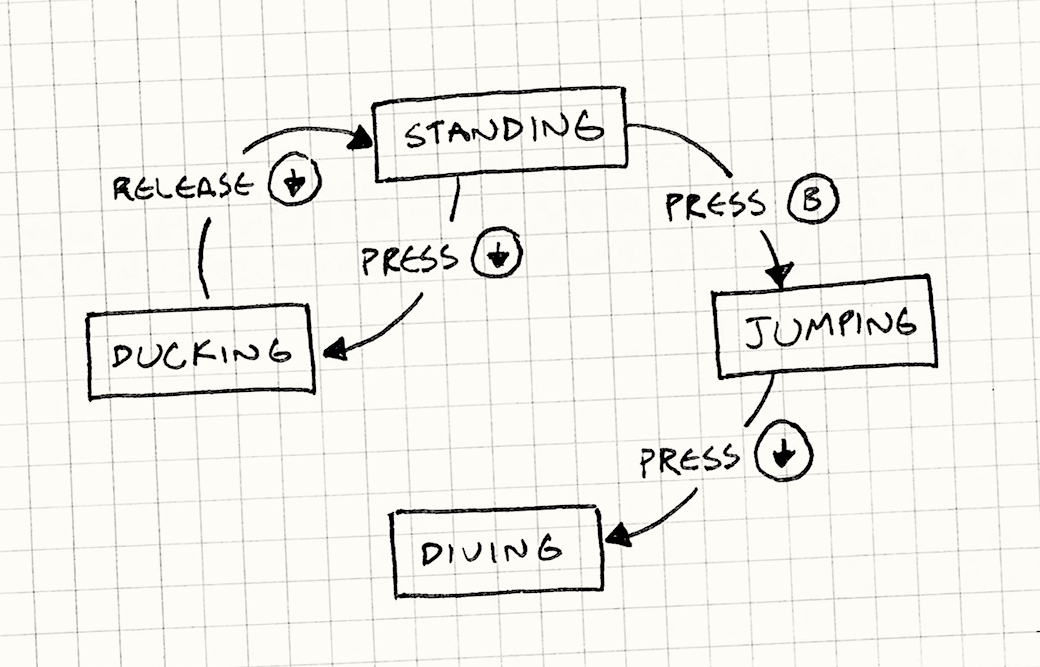
\includegraphics[width=0.5\textwidth]{Images/state_FSM.png}
\end{center}
\caption{Finite State Machine \cite{GameProgrammingPattersFMS}}
\label{pic1}
\end{figure}

Congratulations, we have successfully created an FSM \cite{GameProgrammingPattersFMS}. The idea for this comes from a branch of computer science called \emph{automatic theory}, which includes the famous Turing machine \cite{TuringMachine}. It should be noted that FSMs are the simplest of these kinds of machines. The rules are simple:
\begin{itemize} 
    \item The number of states is fixed. 
    \item The current state can be only one. 
    \item Inputs or events can be sent to the machine. 
    \item Each state has a set of transitions, each of which is associated with an input/event and points to a state.
\end{itemize}

Now that I have introduced FSMs, there's a catch. 
The reason state machines work to untangle complicated code is that they impose a constrained structure on it - they enforce a numbered set of states, only one current state, and hard-coded transitions. However, if you want to create a more complex game AI, you need to work around these issues, and we will look at them in more detail.

\subsection{Concurrent State Machines}

Let us now equip our hero with a weapon. If we want to stick to the constraints of an FSM, we have to double our states: stand, stand with a weapon, jump, jump with a weapon, and so on. It is redundant, but we can add another state to a single machine, namely what the hero is doing and what he is carrying.

\begin{verbatim}
class Hero  {
    private State _state;
    private State _equipment;

    private void HandleInput(Input input) {
        _state.HandleInput(input);
        _equipment.HandleInput(input);
    }
}
\end{verbatim}

\subsection{Hierarchical State Machines}

Thus, if we don't want to repeat our code in all our states, we can define a state that handles several other states. For example, we can create a state \texttt{OnGround} that can handle walking, and other states like running can inherit from walking and add it to their behaviour.

This is called \emph{hierarchical state machine} - states can have superstates, i.e. when an input/event occurs and the current (sub)state cannot handle it, it's passed to the chain of superstates. It can be understood like overwriting inherited methods.

To clarify, if an input/event starts in a sub-state, it's passed on until it's handled by a sub-state - if it's not, it's ignored.

\subsection{Pushdown Automata}

This is an extension of FSMs that uses the concept of stacks. The problem with simple FSMs is that you've no history of previous states. You know what state you're in, but you've no memory of what state you were in.

In FSMs, only one pointer to the current state exists; pushdown automata have a stack of pointers. In an FSM, when you move to the new state, the previous pointer is simply replaced. In pushdown automata, you've a choice:
\begin{itemize} 
    \item Pushes a new state onto the stack, the transition to it occurs, but the previous state isn't discarded, but left just below it. 
    \item Skip the current state, in doing so the state that's under it becomes the new current state.
\end{itemize}

\begin{figure}[h]
\begin{center}
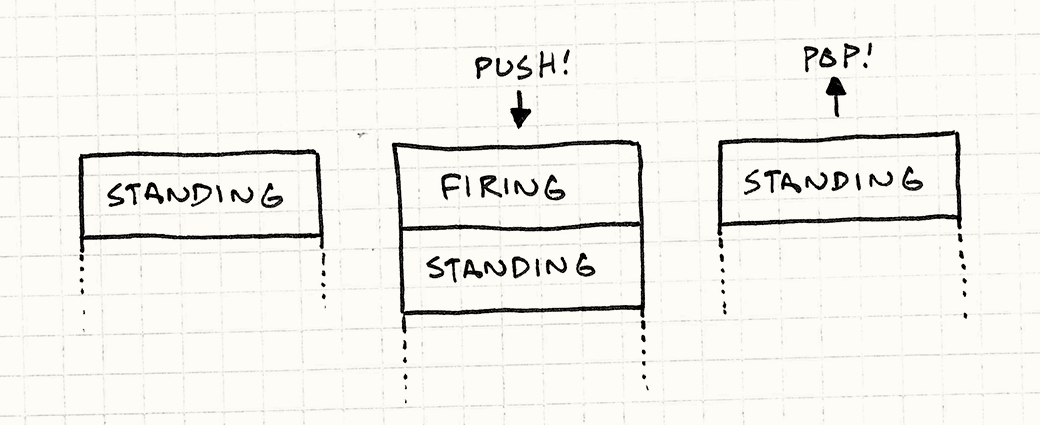
\includegraphics[width=0.6\textwidth]{Images/state_pushdown.png}
\end{center}
\caption{The Pushdown Automata \cite{GameProgrammingPattersFMS}}
\label{pic2}
\end{figure}

\subsection{Example}

Best way to present FSMs is to start with a simple, but upgradable example for future extensibility. To demonstrate this example I will use the Unity \cite{UnitySoftware} editor and engine, also I will use a sprite from a game that I created \cite{KWA}, in the figure \ref{KWA}. It will have a basic state machine with states for: \emph{idle} (grounded), \emph{moving} and \emph{jumping} in the figure \ref{StateMachine}.

\begin{figure}[!hb]
\minipage{0.32\textwidth}
  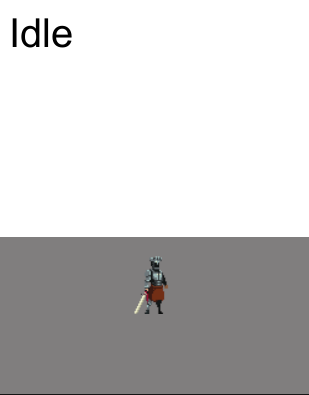
\includegraphics[width=\linewidth]{Images/IdleState.png}
  \caption{Idle}\label{StateFig:Idle}
\endminipage\hfill
\minipage{0.32\textwidth}
  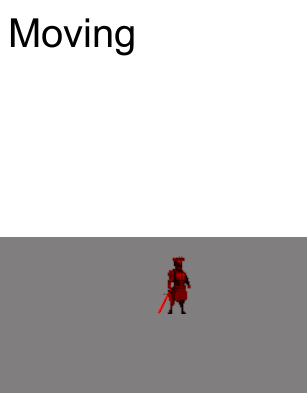
\includegraphics[width=\linewidth]{Images/MovingState.png}
  \caption{Moving}\label{StateFig:Moving}
\endminipage\hfill
\minipage{0.32\textwidth}%
  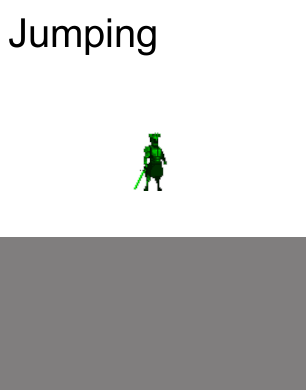
\includegraphics[width=\linewidth]{Images/JumpingState.png}
  \caption{Jumping}\label{StateFig:Jumping}
\endminipage
\label{StateMachine}
\end{figure}

The \texttt{StateMachine} is meant to be overwritten with our movement script. It has a attribute of \texttt{BaseState} and with methods: 
\begin{itemize}
    \item \texttt{Start()} - Sets the current state to the initial state and if there is an initial states, it enters it.
    \item \texttt{Update()} - If there is a current states, it updates the logic in it.
    \item \texttt{LateUpdate()} - If there is a current states, it updates the physics in it.
    \item \texttt{ChangeState(BaseState newState)} - Exits the current state, sets it to the new state and enters the new state.
    \item \texttt{GetInitialState()} - This is a virtual method so we need to override it in our script.
    \item \emph{Misc} - GUI method which displays the current state.
\end{itemize}

The script \texttt{BaseState} is used for all the states our machine can have. It has attributes such as a name and a state machine that it reads. It also has virtual methods that should be overridden: \texttt{Enter()}, \texttt{UpdateLogic()}, \texttt{UpdatePhysics()} and \texttt{Exit()}.

And that's almost it, we have laid the foundation of our state machine, now we just need to implement it for our motion. We create a motion state machine with 3 states: \texttt{IdleState} (which is set as the initial state), \texttt{MovingState}, \texttt{JumpingState}. We have the basic logic for moving in these states and we simply color our sprite each time it enters said state.

\clearpage

\section{Behaviour Trees}

Even with extensions of FSMs, they are quite limited. If the goal is complex game AI, the previous chapter only scratched the surface.

Behaviour Trees (BTs) \cite{BehaviourTreeStarterPack} have proven to be a comprehensive technique for creating fairly versatile AI. They provide a solid foundation to combine other techniques and have full control over behaviour and performance.

To define a BT, you need to know that it is a structure made up of nodes that have different behaviours - individual actions that can be performed. Each node, in turn, has its own subordinate behaviours, which gives the algorithms their tree-like structure. In addition, each behaviour has its own condition that directs the algorithm to its child branches.

\begin{figure}[h]
\begin{center}
    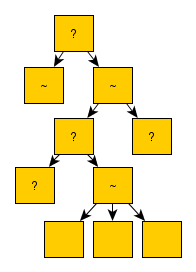
\includegraphics[width=0.35\textwidth]{Images/behaviour_tree.png}
\end{center}
\caption{Behavior Tree \cite{behaviourTreeBlog}}
\label{pic3}
\end{figure}

Every behaviour has its own condition and an action. The algorithm works in such way, that it starts at the root and then for each level it checks the conditions of the behaviours. If a condition matches of a node, it executes the action. None of its siblings will be examined, but its children will. The algorithm \cite{BehaviourSelectionAlgorithms} is as it follows:
\clearpage
\begin{verbatim}
    Make root node the current node
    While current node exists
        Run current node's condition
        If condition returns true
            Add node to execute list
            Make node's child current node
        Else
            Make node's sibling current node
    Run all behaviors on the execute list
\end{verbatim}

The big advantage of BTs \cite{BehaviourSelectionAlgorithms} are their simplicity, since they have no states, their algorithm does not need to know what behaviours are being executed, and behaviours can be written without knowing each other. Extensibility is also a big plus, as it is very easy to add more functions at any time.

But while the BT algorithm is simple and powerful, it is not always the best choice. The algorithm has to start at the root node every time a new behaviour is chosen, which greatly affects runtime compared to FSMs. It also has to deal with a large number of constraints. In addition, memory is an issue since behaviours can be in a loop.

\section{Scripting, the good and the bad}

Now we will talk about the most controversial game AI ever developed. It can turn out to be the best game AI ever or one of the worst - it all depends on its implementation.

However, in order to have a successful scripted AI, it should not be feared. Like any weapon, it should be mastered. 
The architecture of the game can handle scripting techniques in various ways - for the most part, two ideologies \emph{Master and Servant} \cite{ForbiddenScripting} will be used. Although both serve their purpose, it is useful to be clear about what role scripted AI will play in the development of the game.

\subsection{Master and Servant Ideology}

To be successful in developing scripted AI, it is first important to understand how much the AI depends on the overall foundation of the game. The game systems and architecture must be thoroughly thought out in order to develop effective AI. Otherwise, the AI may produce large amounts of errors or even stop development.

Thus, the most viable technique for scripted AI would be the master-and-servant approach. In short, the master script would take care of the high-level aspects of the game, while the servant script would control the general activity of the agents or simply produce some sort of effects. 

\begin{itemize} \item \emph{Master scripts} work best in two scenarios. The first would be when some sort of AI already exists in the game, and then the scripting would simply combine them. But it can also give good results in the other scenario, where it is just scripting. \item \emph{Servant scripts} are best suited when the agent's behaviour needs to be specific. Thus, developers create specific scenarios for each agent, which can lead to excellent results for the environment or background AI.
\end{itemize}

Games, would often tilt to one side or the other. This depends on many circumstances: the experience of the developers, time and budget, the ratio of programmers to designers, etc.

There is a stigma, based on negativity, that gamers cannot enjoy games with scripted AI that have little depth or variety in their AI. However, with the right design and technical background, scripted AI could become a powerful tool with a lot of depth, and players would be grateful for it.

Moreover, scripting should be used in combination with other techniques, because if you rely too much on scripts, you will get a superficial and undesirable AI. On another side, developers must not try to preempt with scripting. This can be avoided by delegation, but the most important thing is to decide on a design early on and stick to it, whether as master or servant. When it comes to scripting, simpler is often better. Rather than designing overly complicated and complex systems, it is better to stick to more flexible and creative solutions.

\subsection{Example}

For scripted AI, there is the perfect example - a game I developed not too long ago using the MonoGame \cite{MonogameDevelopment} framework.
The game \cite{KWA} consists of a knight roaming with his dog, but the dog gets scared by some skeletons and now the knight has to defeat the skeletons to chase and rescue his dog, as shown in Figure \ref{KWA}.

\begin{figure}[h]
\begin{center}
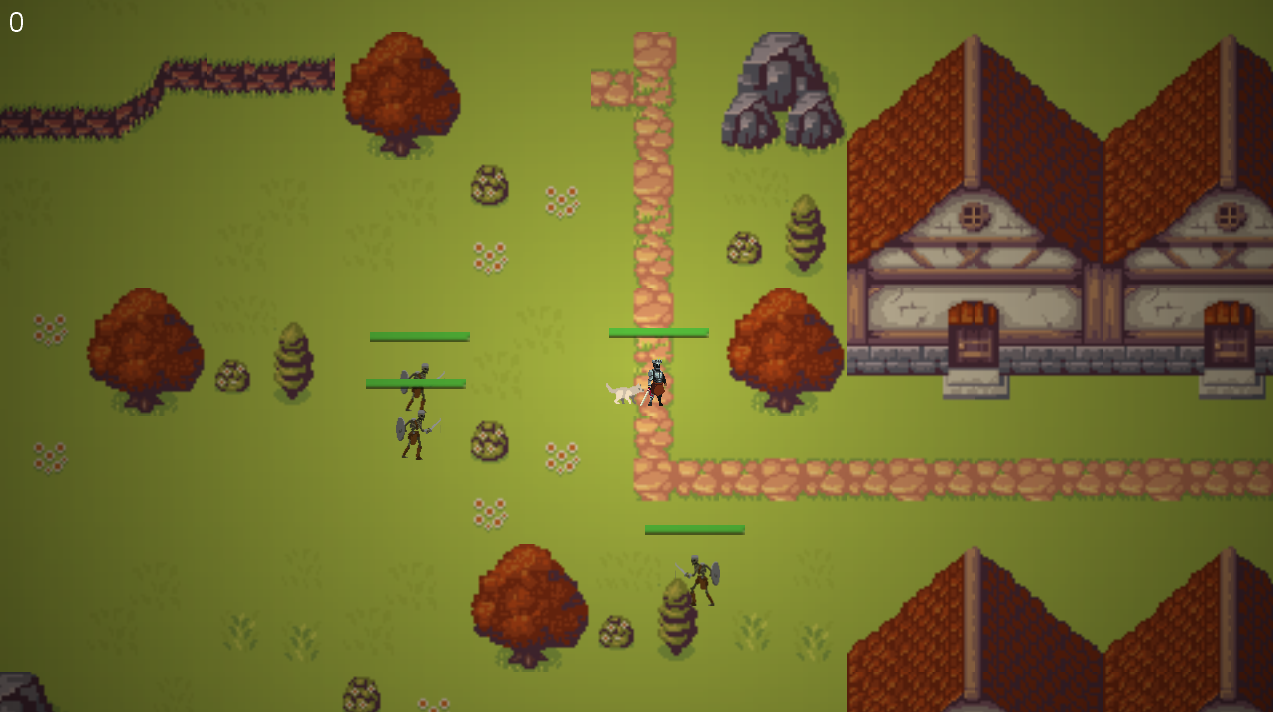
\includegraphics[width=0.5\textwidth]{Images/KWAtown.png}
\end{center}
\caption{Picture of the game with the skeleton enemies}
\label{KWA}
\end{figure}

From this game I wanted to introduce the skeleton AI, because it is the perfect example of scripted AI. Below is an imitation of the code, but the functionality is the same. The skeleton has some private attributes that it uses with its scripted AI.


\lstinputlisting[language={[Sharp]C}, basicstyle=\small]{Code/KWADemo.cs}

This can be an example of scripted servant AI, because many skeletons are spawned and this script is applied to each one. The code is basically only run for the life of the skeleton, and while it is alive, it checks to see if the player is attacking it, and tries to move towards it if it has seen it. If the skeleton is close enough, it will attack.

\section{Fuzzy Logic}

Fuzzy logic \cite{FuzzyAIGames} is an extension of conventional logic that can handle the concept of partial truth between the Boolean dichotomy of \emph{true} and \emph{false}. It usually has its own components such as \emph{fuzzy variables, fuzzy rules and fuzzy interface engines}.

Like the previous techniques, fuzzy logic has the goal of simple design leading to intelligent agents. Controlling a game character with fuzzy logic is easy to implement using appropriate input and output values.

Fuzzy logic is an extension of \emph{crisp logic} (conventional logic), there is the same as binary logic, the variable can be true or false. In crisp logic, the variables can be from a set of two elements, while in fuzzy logic \cite{FuzzyLogicBasedGameSystem}, the concept has been extended to handle partial truth values between true and false. 

For example, weapon range can be divided into melee, ranged, or out of range, as seen in \ref{pic4}.

\begin{figure}[h]
\begin{center}
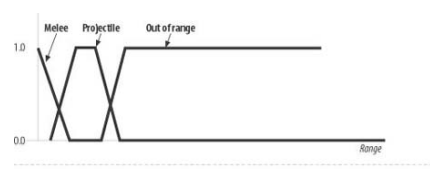
\includegraphics[width=0.53\textwidth]{Images/weapon_range.png}
\end{center}
\caption{Weapon range with Fuzzy Logic \cite{FuzzyAIGames}}
\label{pic4}
\end{figure}

Fuzzy logic offers many advantages for game AI. It can help with NPC decision making or even weapon selection. With its advantages, it can lead to advanced AI with fairly simple implementation. It can even be used in combination with FSMs (when transitioning from one state to another) and BTs (when branching). For example, with conventional logic a car can only brake and accelerate, but with fuzzy logic it is possible to specify how much the car should brake and accelerate based on gradual behaviour. 

\subsection{Pitfalls}

As good as fuzzy logic sounds so far, I must also talk about its drawbacks. Due to its knowledge-based nature, it requires proper definition of input and output variables and their relationships. Another disadvantage is that the system of fuzzy logic, if not carefully designed, may result in many rules being checked at any given time, thus losing the advantage of low computational cost.

In a video game, there may be many input variables for an agent's behaviour, each of which has its own number of fuzzy sets. For this reason, the fuzzy rules can grow exponentially and it could even lead to a combinatorial explosion \cite{CombinatorialBombing}.

\section{Flocking}

Flocking is a technique used to simulate the intelligent movement of groups, the groups are called \emph{boids}. It is most often used when NPCs must move in a cohesive unit rather than independently. The game genre that most often uses this technique is RTS (real-time strategy) games. The name "flocking" comes from "flock of birds".

Craig W. Reynolds is responsible for the flocking algorithm with his groundbreaking research \cite{FlocksReynolds}. His implementation is leaderless, i.e., no bird leads the flock, but all simply follow the group, which seems to have a mind of its own.

Flocking behaviour can be simulated using three principles \cite{FlockingBehaviour}, see figures \ref{fig:image3}, \ref{fig:image2}, \ref{fig:image1} \cite{WebsiteBoids}: 
\begin{itemize} 
    \item \emph{Alignment} - Tracks the average speeds of the boids and tries to keep the average speed. 
    \item \emph{Cohesion} - Calculates the direction of the average position of the boids and tries to direct all boids to stay together as a group. 
    \item \emph{Separation} - Each boid knows the distances of its neighbours and tries to use this knowledge to exert a repulsive force in the opposite direction to maintain distance from them. In a sense, it is collision avoidance within the flock.
\end{itemize}

\begin{figure}[!htb]
\minipage{0.27\textwidth}
  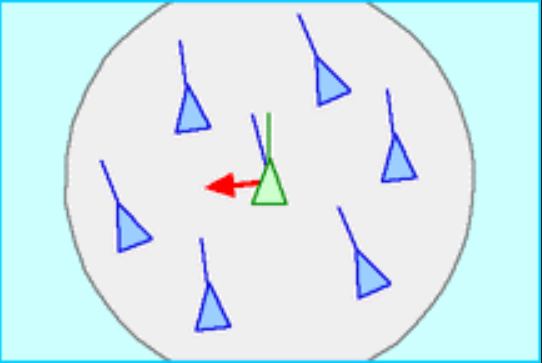
\includegraphics[width=\linewidth]{Images/alignment.png}
  \caption{Alignment \cite{WebsiteBoids}}\label{fig:image3}
\endminipage\hfill
\minipage{0.27\textwidth}
  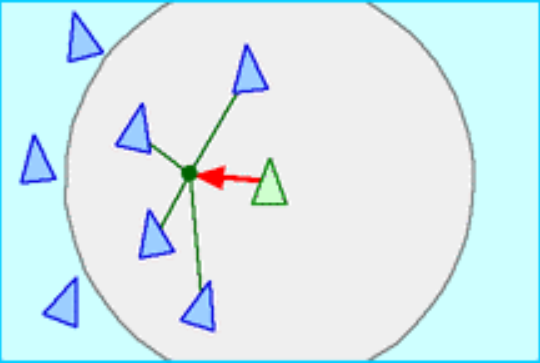
\includegraphics[width=\linewidth]{Images/cohesion.png}
  \caption{Cohesion \cite{WebsiteBoids}}\label{fig:image2}
\endminipage\hfill
\minipage{0.27\textwidth}%
  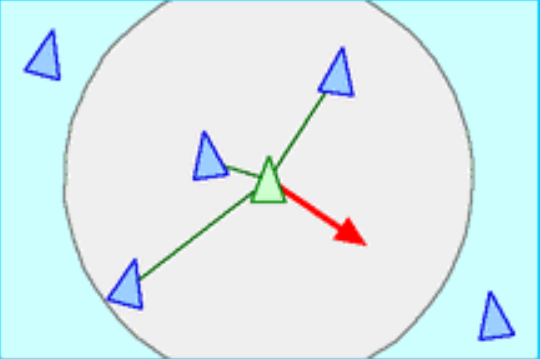
\includegraphics[width=\linewidth]{Images/separation.png}
  \caption{Separation \cite{WebsiteBoids}}\label{fig:image1}
\endminipage
\label{pic5}
\end{figure}

The path of boids that want to move is computed using the A* pathfinding algorithm \cite{AStarHart1968}. Its simple goal is to find the shortest path from point A to point B. It is a well-known method that can be used as a basis for pathfinding problems because of its simplicity, efficiency, and modularity.

But the A* algorithm is not foolproof, in many cases an additional algorithm or a modification of the core mechanics is required. Also, A* can find a path much faster than other search methods, but it is not guaranteed that the result will be the shortest path. Research has shown that A* produces a correct result only 85\% of the time \cite{FOEAD2021507}. Overall, the traditional algorithm cannot keep up with modern pathfinding requirements, so game developers need to optimise and strengthen it for adequate results.

\clearpage

\subsection{Example}

The technologies I will use to present the example are again the Unity \cite{UnitySoftware}editor and the Unity engine. This implementation is based on Craig Reynolds' program \cite{FlocksReynolds} for simulating flocking behaviour. So the way the example works is that each boid controls itself by separation, cohesion, and alignment each time \texttt{Update()} is called. So that means it's pretty expensive, but it's quite sufficient for a demonstration. Most of the time it has a time complexity of $ \mathcal{O}(n^2) $.

\begin{figure}[h]
\begin{center}
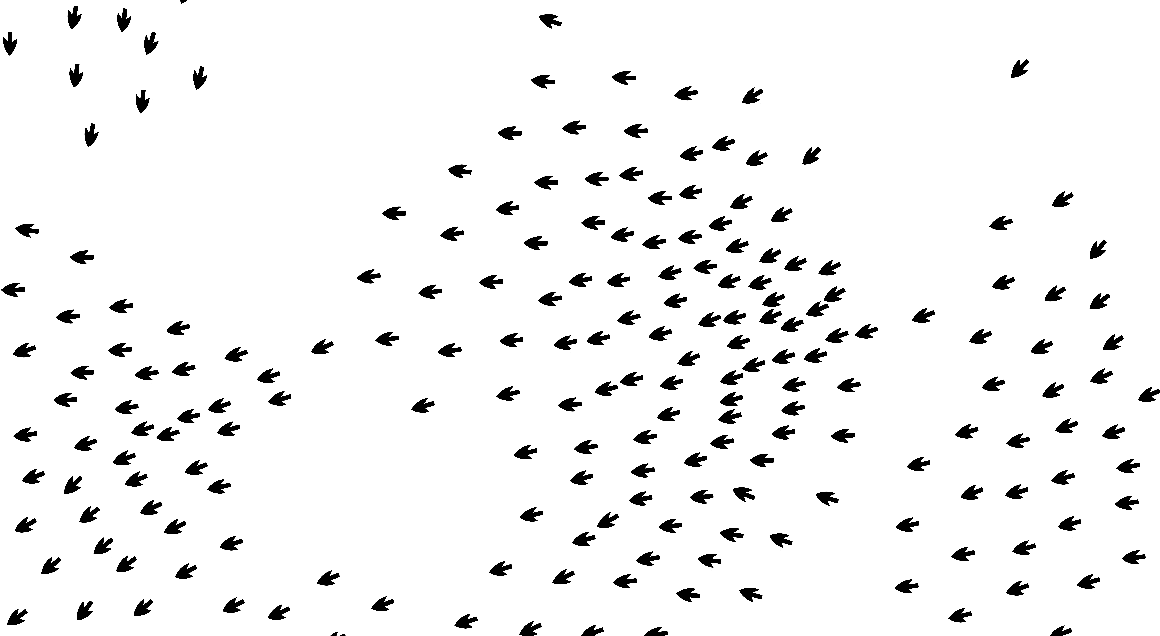
\includegraphics[width=0.6\textwidth]{Images/FlockingExample.png}
\end{center}
\caption{Flocking example with 200 boids}
\label{100boids}
\end{figure}

We can start with 200 boids at first in figure \ref{100boids}, we can see that right away they formed two flocks, but later on disperse. So, we have three methods for calculating alignment, cohesion, separation amount, the rules for the algorithm them are:
\begin{itemize}
    \item \texttt{Alignment()} - takes care of the flock's average velocity.

\lstdefinestyle{sharpc}{language=[Sharp]C, basicstyle=\small}
\lstset{style=sharpc}
% Alignment code ------
\begin{lstlisting}
var velocity = Vector2.zero;
foreach (var boid in boids)
{
    velocity += boid.velocity;
}
velocity /= boids.Count();
var steer = (velocity.normalized * maxSpeed) - velocity;
return steer;
\end{lstlisting}
% Alignment code ------

    \item \texttt{Cohesion()} - takes care of the flock's direction - each boid moves to the center of mass of its neighbours.

% Cohesion code ---------
\begin{lstlisting}
var sumPositions = Vector2.zero;
foreach (var boid in boids)
{
    sumPositions += boid.Position;
}
var average = sumPositions / boids.Count();
var direction = average - Position;
var steer = (velocity.normalized * maxSpeed) - velocity;
return steer;
\end{lstlisting}
% Cohesion code ---------

    \item \texttt{Separation()} - boids attempt to move away from the neighbours of a certain radius who are too close.

% Separation code ---------
\begin{lstlisting}
var direction = Vector2.zero;
boids = boids.Where(DistanceTo(o) <= neighborhoodRadius / 2);
foreach (var boid in boids)
{
    var difference = Position - boid.Position;
    direction += difference.normalized / difference.magnitude;
}
direction /= boids.Count();
var steer = (direction.normalized * maxSpeed) - velocity;
return steer;
\end{lstlisting}
% Separation code ---------

\end{itemize}

Then we get the final acceleration, which is calculated as the weighted sum of the results of these three methods \texttt{alignmentSteer * alignment + cohesionSteer * cohesion + separationSteer * separation}.

While this example for flocks \cite{FlocksReynolds} has focused on movements similar to those of fish or flocks of birds, the algorithm can be extended to express movements of other animals. Realism can be increased by adjusting the parameters of the algorithm.

\section{Genetic Algorithm}

A genetic algorithm \cite{GameAIGeneticAlg} is a probabilistic algorithm that generates an approximate solution based on Darwin's theory of evolution. The basic idea of the algorithm is to generate new offspring from an existing population and then select the fittest offspring from that population for the next generations. This algorithm has been around for several decades, so there can be many variations.

In this section we'll take a look at one particular genetic algorithm for which we need to define some terms:

\begin{itemize}
    \item \emph{Gene} - Single parameter of search space
    \item \emph{Chromosome} - Collection of genes
    \item \emph{Individual} - Instantiated chromosome
    \item \emph{Population} - Collection of individuals
    \item \emph{Fitness} - Evaluation of an individual in our selected problem
    \item \emph{Crossover} - Process to create a new individual by breeding two
    \item \emph{Mutation} - Process to randomly change some genes to oppose local optima (solution that is optimal within a neighboring set of candidate solutions \cite{LocalOptimum}) 
    \item \emph{Generation} - One iteration of the Genetics Algorithm
\end{itemize}

\clearpage

Now, that we have defined some general terms we need for the algorithm \cite{GameAIGeneticAlg}, we can go ahead and get into it:

\begin{verbatim}
    Generate an initial random population
    Calculate fitness of every individual of the population
    Copy the individuals with high fitness to next generation
    Randomly mutate genes of individuals in current generation
    From the mutated generation, choose pairs of individuals 
        with certain fitness to crossover
    If the number of maximum iterations of generation is not 
        reached, go the second line
\end{verbatim}

With a probabilistic algorithm, it is best to iterate until there are no more improvements, but with the genetic algorithm, we need to set up a certain number of iterations because it is always mutating.

The benefit of genetic algorithms is immense because it can robustly and effectively search an insufficient search space when we have little knowledge. It is best suited for nonlinear problems. The appeal of this algorithm comes from its elegance and simplicity for its ability to discover good solutions to high dimensional problems \cite{CurrentAIGames}.

The downside is that genetic algorithms require high computational and memory capacity, so they are at a major disadvantage when playing a game. Game developers can get around this primarily by running the algorithm when the game is not being played. In summary, it is an effective algorithm based on evolution and natural selection used for learning and optimization.

\chapter{ML-Agents}
\label{ch3}

\section{Technologies}

In order to use the ML-Agents toolkit correctly, we need certain technologies. If we want to use the ML-Agents toolkit with Unity, we should start with the Unity editor and the Unity game engine \cite{UnitySoftware}. Then we should install "ML Agents" in Unity Package Manager.

After that we should have (or install) Python \cite{PythonManual} (I used Python 3.9). With python pip we need the packages pytorch (\texttt{torch}) and \texttt{mlagents} - For this step I decided to use a virtual environment, which is advantageous to have the right versions and to better organize the setup.

With the \texttt{mlagents-learn} command and Unity open, we can now enter the chapter with ease.

\section{Background}

After looking at some of the major game AIs used in the industry, I'd like to introduce an open source project, the Unity Machine Learning Agents Toolkit, or ML-Agents Toolkit \cite{MLAgents}. Using a Python \cite{PythonManual} API, it trains intelligent agents through \emph{reinforcement learning, imitation learning, neuroevolution}.

\subsection{Agents}

The technology of ML-Agents is mainly used for training agents which are basically NPCs, we can use a variety of methods for training. To start using ML-Agents, we should explain what agents are:

\begin{itemize} 
    \item \emph{Observations} - How the agent sees the environment, they can be numerical and/or visual. Numerical observations can be some kind of attributes from the environment (they can be discrete or continuous), for the best results the agent should have several continuous numerical observations. Observations can also be visual and come from the agent's cameras. They are separated from the environment so that the agent cannot be confused with data from the whole game/environment. 
    \item \emph{Actions} - What can the agent do, just like the observations, the actions can be discrete or continuous. They can become as complex as the environment allows. 
    \item \emph{Reward signals} - How well the agent does, these signals do not need to be sent at all times. The agent should only be rewarded when it does something good, and punished when it does something bad. It should be noted that the reward is how the agent's goal is communicated, so it should be set up optimally for the best results.
\end{itemize}

\subsection{Architecture}

The ML-Agents Toolkit system works with 5 interconnected high-level components. And these are:

\begin{itemize} 
    \item \emph{Learning environment} - is actually the Unity scene and all game objects. This scene is used for either training or testing environments. This is where the Unity package ML Agents mentioned above comes into play. It is used to define the agents and their behaviour. 
    \item \emph{Python low-level API} - interacts and manipulates the learning environment, it lives outside the learning environment and interacts with it via the External communicator. 
    \item \emph{External communicator} - is used for the connection between the environment and the Python API. 
    \item \emph{Python trainers} - the place where the ML algorithms are stored, which are included in the \texttt{mlagents} package. 
    \item \emph{Gym wrapper} \cite{openAIGym} - the common technology used to interact with environments.
\end{itemize}

\begin{figure}[h]
\begin{center}
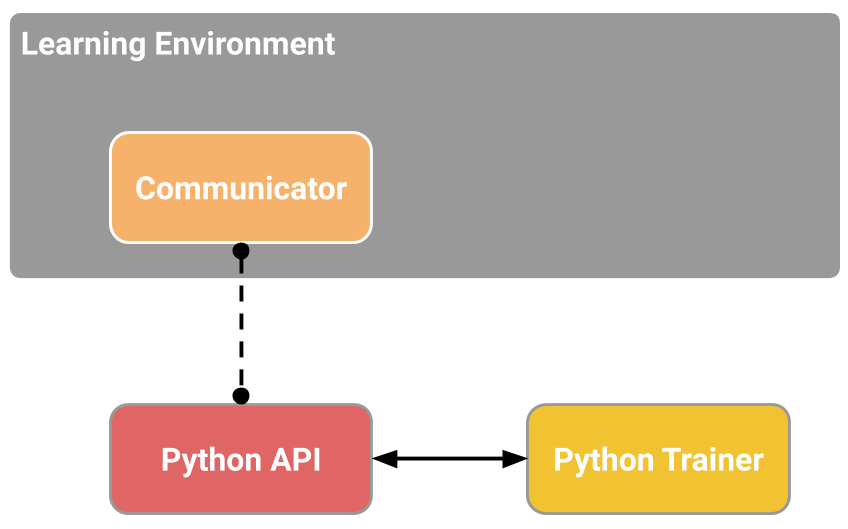
\includegraphics[width=0.7\textwidth]{Images/learning_environment_basic.png}
\end{center}
\caption{Simplified ML-Agents architecture \cite{MLAgents}}
\label{pic6}
\end{figure}


\clearpage

The learning environment in the Unity scene consists of two components:
\begin{itemize} 
    \item \emph{Agent} - is linked to the game object, manages the observations, actions and rewards. 
    \item \emph{Behaviour} - defines the attributes and the number of actions that the agent can perform. It is like a method that collects observations and rewards and returns actions. It can be: 
    \begin{itemize} 
        \item \emph{Learning} - undefined, in the process of being trained. 
        \item \emph{Heuristic} - is defined by hard-coded rules, used mainly as input for controlling the agent. \item \emph{Inference} - is already trained and contains an already working and trained neural network file. 
    \end{itemize} 
    Basically, after a learning behaviour is trained, it becomes an inference behaviour.
\end{itemize}

With this knowledge of the architecture of ML agents, we can represent what a game would look like.

\begin{figure}[h]
\begin{center}
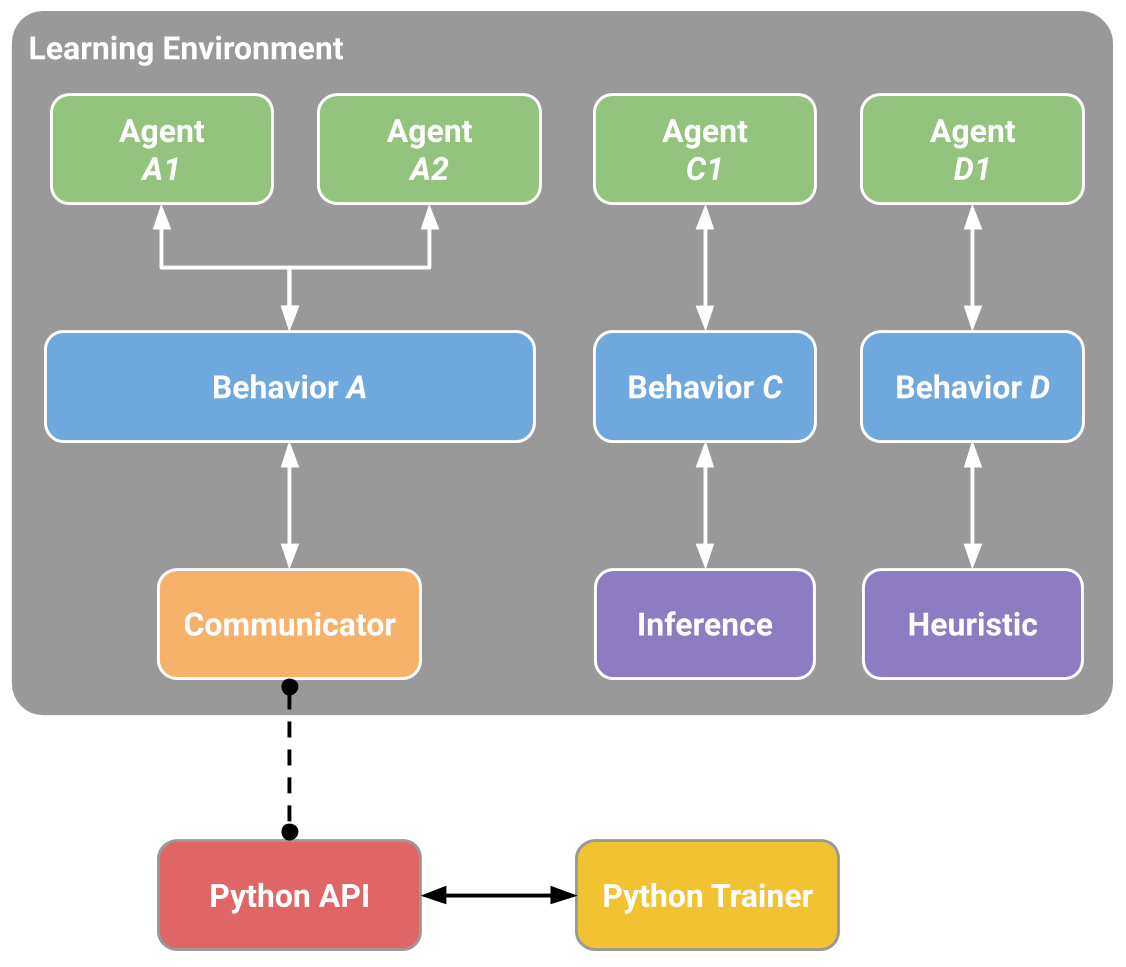
\includegraphics[width=0.5\textwidth]{Images/learning_environment_example.png}
\end{center}
\caption{Example of how the architecture looks of a simple game \cite{MLAgents}}
\label{pic7}
\end{figure}

\subsection{Training methods}

Before I go into the examples, I would like to give a brief overview of the ML algorithms that are part of ML agents.

\subsubsection{Note on reward signals}

A quick note is that rewards in ML-Agents can be either \emph{intrinsic} or \emph{extrinsic}. Rewards that the agent can receive from the learning environment are called extrinsic. However, rewards can also be defined extrinsically from the environment; we refer to these as intrinsic rewards.

The toolkit allows reward signals to be customised in four ways:
\begin{itemize} 
    \item \texttt{extrinsic} - represents the rewards in the environment that are enabled by default. 
    \item \texttt{gail} - represents the intrinsic rewards defined by GAIL (we will look at it below) 
    \item \texttt{curiosity} - represents the intrinsic rewards that encourage the player to explore, it is defined by a curiosity module 
    \item \texttt{rnd} - represents the intrinsic reward that encourages the player to explore; it is defined by a curiosity module
\end{itemize}

\subsubsection{Deep Reinforcement Learning}

The package implements two algorithms, Proximal Policy Optimization (PPO) and Soft Actor-Critic (SAC). The default is PPO, as it has been shown to be more general and stable. On the other hand, we had SAC, which tends to accumulate a number of experiences and learn from them. So from the efficiency point of view, PPO would require more sampling, so SAC is a better choice for heavier environments. Also, SAC promotes exploration since it is a "maximum entropy" algorithm.

The curiosity reward signal we mentioned earlier is managed by the Intrinsic Curiosity Module. It is an implementation in ML-Agents, which is from "Curiosity-driven Exploration by Self-supervised Prediction" \cite{CuriosityExploration}. While we are on the subject, RND, which is \emph{Random Network Distillation} \cite{ExplorationRND} is also a module in ML-Agents that helps agents explore.

\subsubsection{Imitation Learning}

Often agents have difficulties at the beginning of training. To prevent or help this process, the desired behaviour can be demonstrated to the agent so that it can learn from it instead of trying it over and over again. This is called imitation learning, and better yet, it can even be combined with the reinforcement learning that already exists. This drastically decreases the time it takes for the agent to learn the behaviour.

For imitation learning, ML-Agents uses behavioural cloning and generative adversarial imitation learning. In order for the agents to learn through demonstrations, GAIL and BC must be enabled in the appropriate \texttt{yaml} configuration file.

Demonstrations can be recorded in the Unity editor or saved as assets for later use.

\begin{itemize} 
    \item \emph{GAIL} or \emph{Generative Adversarial Imitation Learning} \cite{GAIL} uses an adversarial approach to reward the agent for using actions similar to those in the demonstrations. It works well with a limited number of demonstration instructions and has a second neural network, \emph{discriminator}, that distinguishes whether an action or observation comes from the demonstration or is generated by the agent itself. Note: The GAIL method actually encourages the agent to stay as long as possible due to \emph{survivor bias} \cite{SurvivorBias} in the learning process. Therefore, it is best to stick to a low strength GAIL. 
    \item \emph{BC} or \emph{Behavioral Cloning} encourages the agent to adhere strictly to the demonstrations; this works best when the demonstrations include every state the agent can take. The best results are obtained when combining GAIL and BC.
\end{itemize}

To conclude this subsection: Imitation learning with ML agents is very powerful and should be used in certain ways. BC is best used on its own or as a step before training with GAIL and/or RL. RL can be used alone (either with algorithm PPO or SAC) or in combination with BC and/or GAIL. This can lead to quite amazing results, as we will see in the next section.

\section{Examples and usages}

Now that we know essentially how the toolkit works, I can present some examples of how to use it.

\subsection{Move to goal}

Let's start with a simpler example to understand how the technology is used in practice. The goal of this first example is to train the agent to move to a yellow ball (the goal). The scene consists of an agent, a goal, and walls and looks like the scene in figure \ref{pic8}.

\begin{figure}[h]
\begin{center}
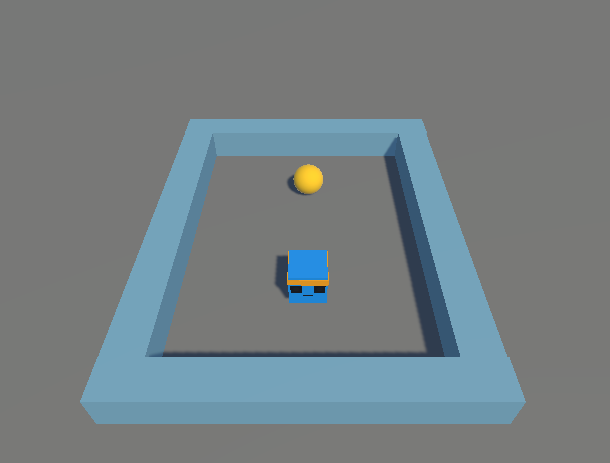
\includegraphics[width=0.5\textwidth]{Images/MoveToGoal.png}
\end{center}
\caption{Move to goal scene}
\label{pic8}
\end{figure}

The first thing we need to do is create an agent script component, which would inherit from the class \texttt{Agent}. Our class would only have to know the position of the goal (it would be a Serialized Field), from the parent class we would need to override the following methods:
\begin{itemize}
    \item \texttt{OnEpisodeBegin} - Every time an episode finished this method is called, so the positions of the goal and agent should be reset. Note: If we reset to the same position every time, the model will become over fitted only move to the same position of the goal (even if we move it). In order to avoid this, it should reset to a random position.
    \item \texttt{CollectObservations} - this method takes a sensor parameter with the class \texttt{VectorSensor}, here the positions of our agent and goal should be added.
    \item \texttt{OnActionReceived} - its plan to take continuous numeric data for the movement of the x axis and z axis, so in this method through the parameter with the class \texttt{ActionBuffers} we can take the before mentioned data and move our agent.
    \item \texttt{Heuristic} - this method works only if the agent's behaviour is set to Heurstic only mode and in our case, its used to test the environment if it works properly.
\end{itemize}

Now we can add the script component to our game object and it should look something like the figure \ref{pic9}.
\begin{figure}[h]
\begin{center}
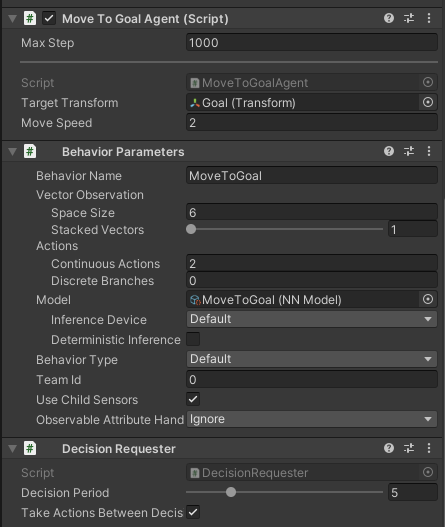
\includegraphics[width=0.35\textwidth]{Images/movetogoalcomponent.png}
\end{center}
\caption{Move to goal agent component}
\label{pic9}
\end{figure}

To optimize learning, the environment should be placed in a prefab and instantiated several times in the scene for better learning results. When we are done learning, we can use only one environment.

Now we should specify when the episode ends and the agent gets a positive reward: when it touches the target. 
And the episode ends and the agent gets a negative reward: when he touches the walls.

In the figure \ref{pic9}, the first thing that stands out is the maximum step. It indicates how many steps the episode can take before it ends. It is environment specific so that the episode resets and the agent is not motivated to stay in one place only to get the best reward. Next, the continuous actions are set to two, since that is how we move our agent (in the two axes). We also had to add a decision requester and that's it.

Finally, we need to run the commands to train our agent with \texttt{mlagents-learn MoveToGoal.yaml --run-id=MoveToGoal}. For this example, we do not really need to change the configuration file - the default parameters should work fine. Note: We can use the \texttt{tensorboard --logdir} command to see how our model progresses in our environment (see figure \ref{pic10}).

\begin{figure}[ht]
\begin{center}
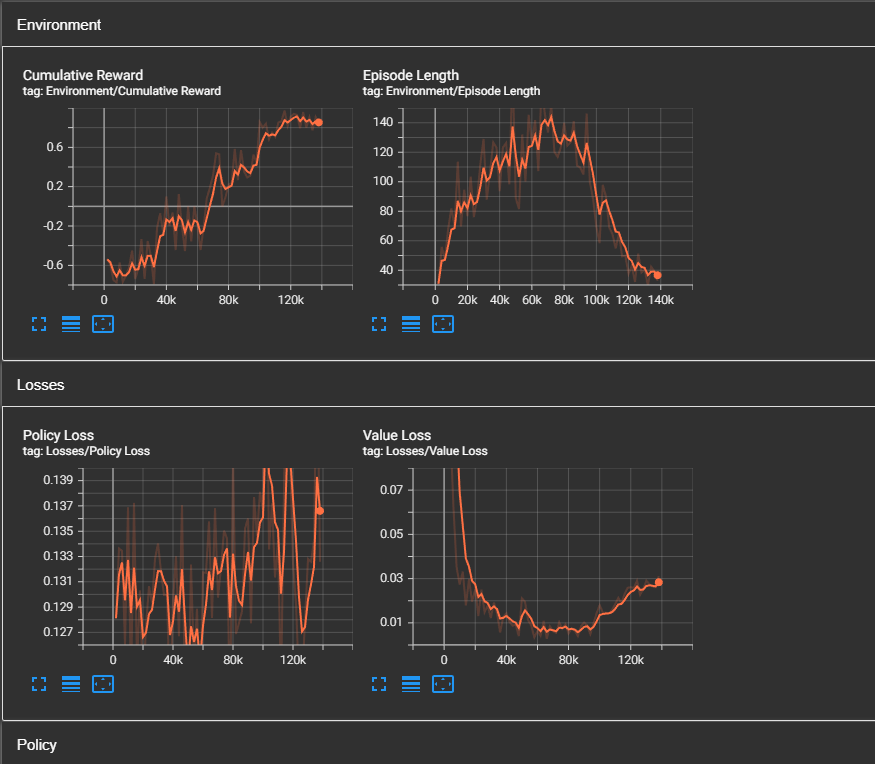
\includegraphics[width=0.4\textwidth]{Images/tensorboard.png}
\end{center}
\caption{Tensorboard of MoveToGoal example}
\label{pic10}
\end{figure}

If we see good progress, we can move on and stop learning. The model is saved in an \texttt{.onnx} (Open Neural Network Exchange Format) file that we can use later for a brain (model). And that's basically it, we have successfully trained our first NN model, we can use this brain for any purpose.

\subsection{Dungeon escape}

I would like to introduce the next example of ML -agent performance and show what it is capable of. This game is one of the many ML-Agents \cite{MLAgents} examples, it is a simple game where players have to escape from the dungeon by taking the key and unlocking the door while being guarded by a dragon.

\begin{figure}[h]
\begin{center}
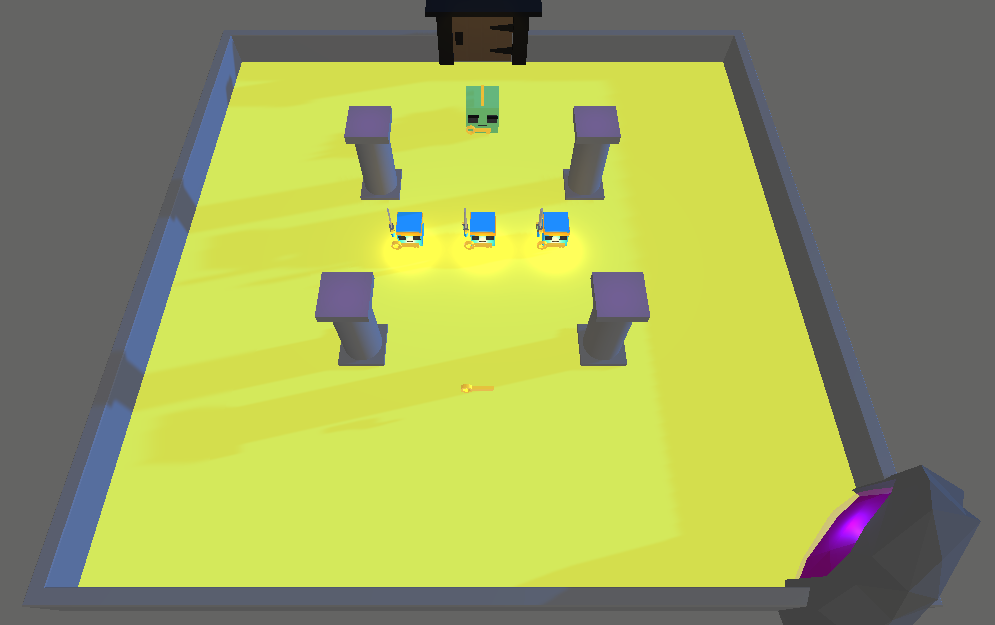
\includegraphics[width=0.5\textwidth]{Images/DungeonEscape.png}
\end{center}
\caption{Dungeon escape example \cite{MLAgents}}
\label{pic11}
\end{figure}

What is interesting for this example is that the agent uses a 3D ray perception sensor (see figure \ref{pic12}) and its observations are visual, rather than numeric.

\begin{figure}[h]
\begin{center}
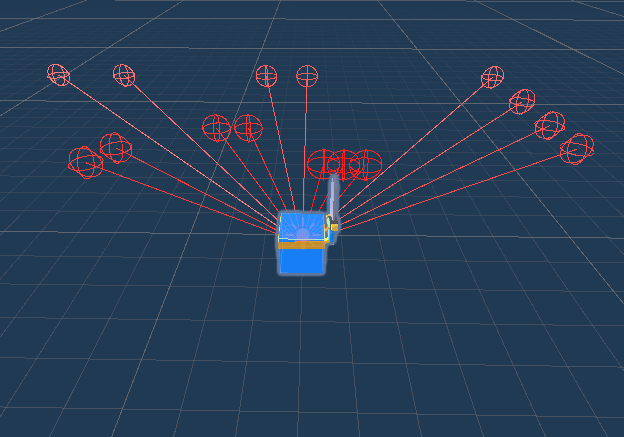
\includegraphics[width=0.3\textwidth]{Images/AgentDungeonEscape.png}
\end{center}
\caption{Ray perception sensor on an agent}
\label{pic12}
\end{figure}

This examples takes use of the \texttt{SimpleMultiAgentGroup} and the agents register to it (the agents are our knights in the figure \ref{pic11}). The agents take 6 discrete actions, two for rotation and four for direction movement. They can pick up a key and if they have it they can unlock the door and get a reward. Or if an agent collides with the dragon, both the dragon and the agent die.

\subsection{Pyramids}

This example is similar to the previous one, the agent is the same but we only have one here, see figure \ref{fig:PyramidPicture}. So, the goal here is for the agent to press a button, when it presses the button a pyramid with a green block on top spawns. When it touches the green block, it wins.

\begin{figure}[ht]
\minipage{0.45\textwidth}
  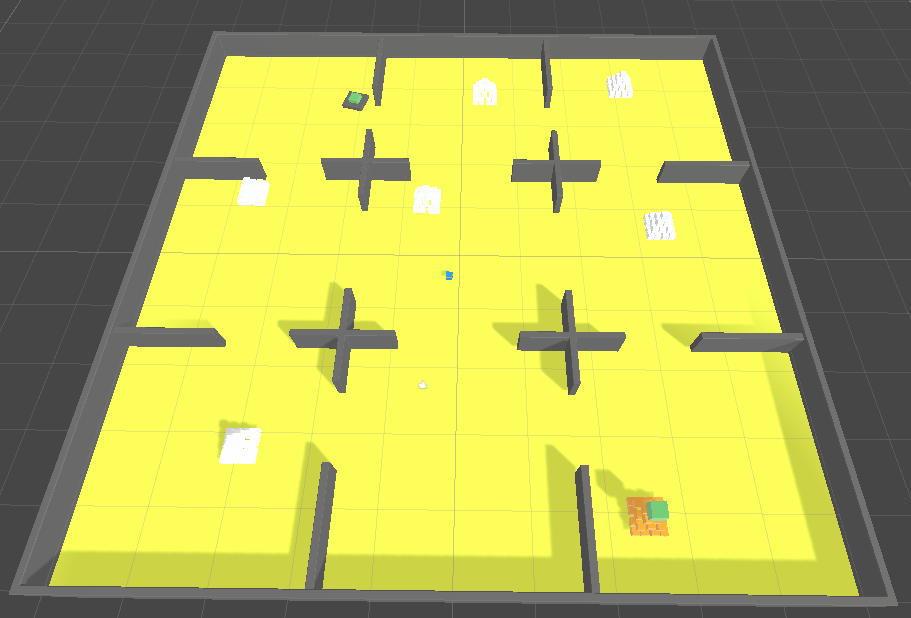
\includegraphics[width=\linewidth]{Images/PyramidsExample.png}
  \caption{Pyramids example \cite{MLAgents}}\label{fig:PyramidPicture}
\endminipage\hfill
\minipage{0.45\textwidth}
  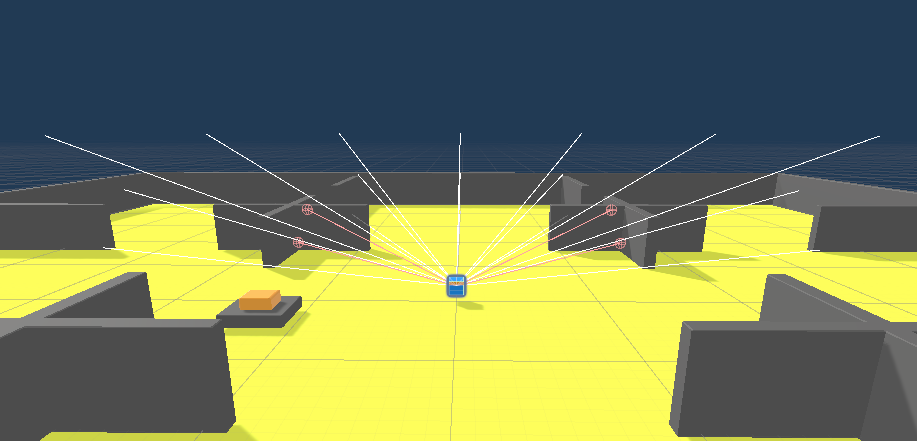
\includegraphics[width=\linewidth]{Images/PyramidsRaycast.png}
  \caption{Raycasts of the agent}\label{fig:PyramidRaycasts}
\endminipage\hfill
\label{PyradmidsExample}
\end{figure}

The agent's observations are ray-casts detecting the environment and the state of the button switch. The ray-casts detect the walls, pyramids, green blocks and the switch, and with a reward of 2 every time the agent touches the green block. It can successfully train to search and find the switch, turn it on and go break down the pyramid with the green block. Also, it should be noted that the agent gets a negative reward $ -1 / MaxStep $ on every step so the evnironment can show urgency to it.

\subsection{ML Car}

So as the saying goes, we saved the best things for last. In this example, we will show the power of the library of ML-Agelts \cite{MLAgents} in self driving cars. The goal here is to create self driving agents which know how to race in a specific track (environment).

First things first, we need to create a car. We start off by modeling a simple car and then creating a script called \texttt{CarController}. All that the script does is use the \texttt{RigidBody} of the model car to simulate movement with a simple method \texttt{SetInput(float moveInput, float turnInput)} - because that's all we need for movement.

Next up, we should create some kind of system for tracking the progress of our car. I created a simple checkpoint system, check figure \ref{CarWithCheckpoints}. The checkpoints keep track of the cars in the scene, and they must be passed in order - this is to create progress of the track. Also, I created much needed events for when passing the correct checkpoint and wrong checkpoint which will come in use later.

\begin{figure}[h]
\begin{center}
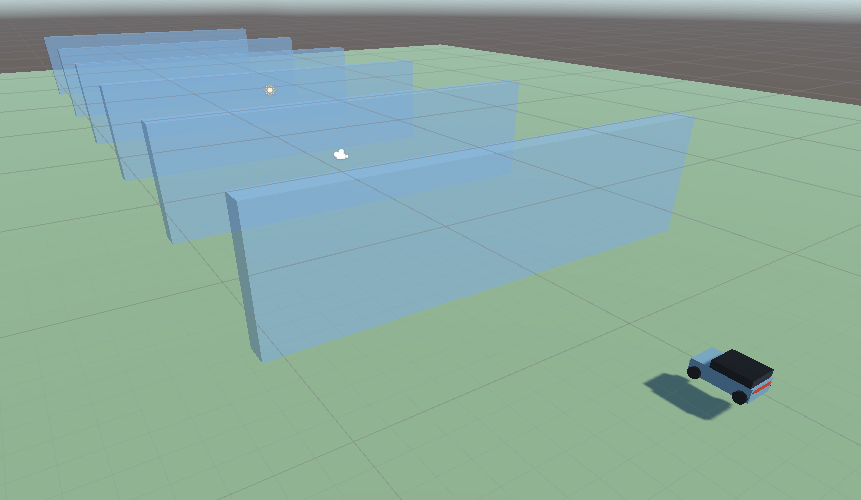
\includegraphics[width=0.7\textwidth]{Images/CarWithCheckpoints.png}
\end{center}
\caption{Model car with checkpoints}
\label{CarWithCheckpoints}
\end{figure}


\subsubsection{Car agent}

Now that we created the basics of our game, we should go on in the implementation of ML-Agents on our agent. For our actions, our agent uses 2 discrete branches of size 3 for each possible movement - turns: left, straight, right - directions: forward, in place, backward. For observations, the agent gets the directions of the next checkpoint. But that is not all, the agent is equipped with a 3D raycasts, see figure \ref{CarAgent}, which are there  to only spot walls and checkpoints. The configuration of training is also not complicated, we just need to mind the number of steps the agent has to take in an episode, which in our case that number needs to be high.

\begin{figure}[h]
\begin{center}
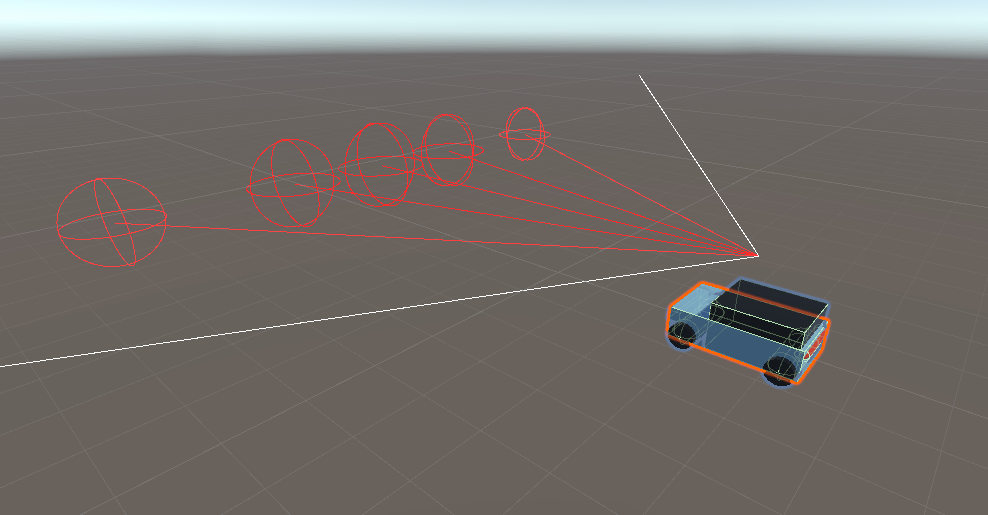
\includegraphics[width=0.7\textwidth]{Images/CarAgent.png}
\end{center}
\caption{Car Agent}
\label{CarAgent}
\end{figure}

\subsubsection{Straight track}

To begin with, I created a simple straight track to test how the agent behaves, see figure \ref{StraighTrack}. When every episode ends, every agent is spawned at the spawn location with a little offset on x and y axis. Also, there are red walls, when the agent touches them it gets a negative reward and the episode restarts. But, when the agent crosses a checkpoint which is not a wrong one in progression order, it gets rewarded.

When the training started, results were almost immediate. With training for a minute or two, it generated a good result (brain), it could finish our simple straight track with ease. Interesting thing is that at the end is an empty space and the agents were searching for checkpoint, which there was none.

\begin{figure}[h]
\begin{center}
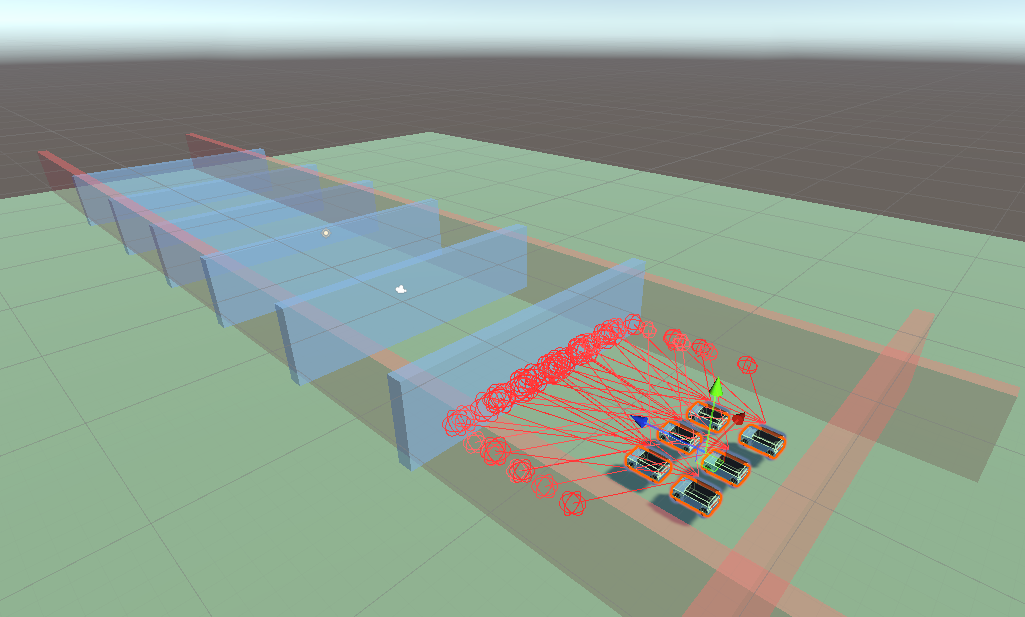
\includegraphics[width=0.5\textwidth]{Images/StraightTrack.png}
\end{center}
\caption{Straight track with 6 agents}
\label{StraighTrack}
\end{figure}

\subsubsection{Circle track}

Next up is a circular track, see figure \ref{CircleTrack}. With 10 agents, they trained pretty fast and in no time a brain was produced that can circle around the track indefinitely. Main problem was here setting up the checkpoints in the turns. Now we concluded that the agent can handle only left turns pretty consistently, next up would be something more problematic.

\begin{figure}[h]
\begin{center}
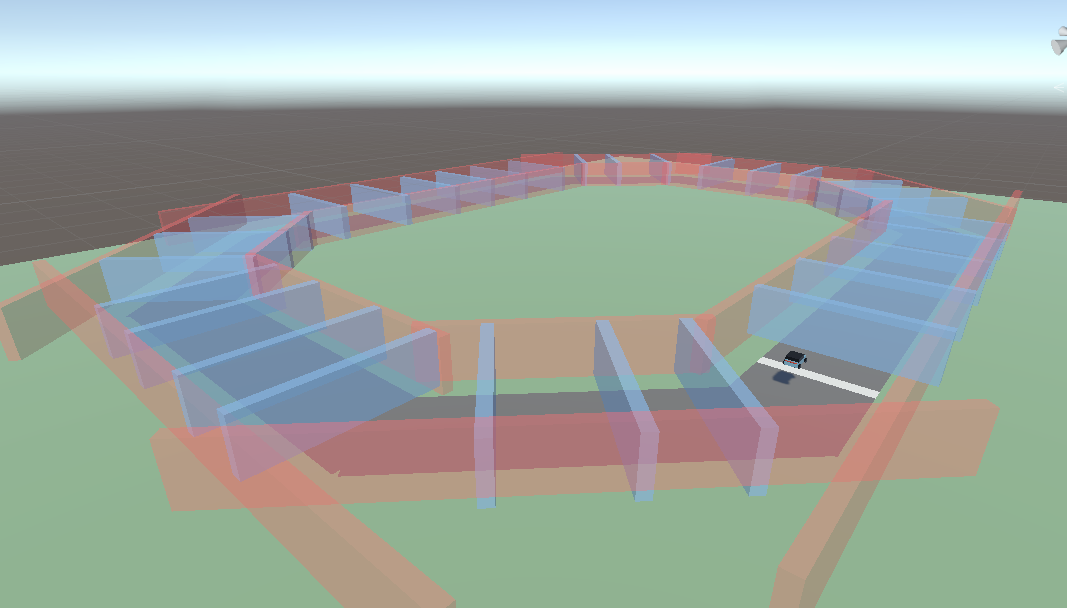
\includegraphics[width=0.5\textwidth]{Images/CircleTrack.png}
\end{center}
\caption{Circular track}
\label{CircleTrack}
\end{figure}

\clearpage

\subsubsection{Sprint track}

For my last example, I decided to create a track to test the turning of the agent, see figure \ref{SprintTrack}. Also, for this example I used Imitation Learning, which was explained above. For that, I created a demonstration of me driving the car through the track for the agent to later use.

\begin{figure}[h]
\begin{center}
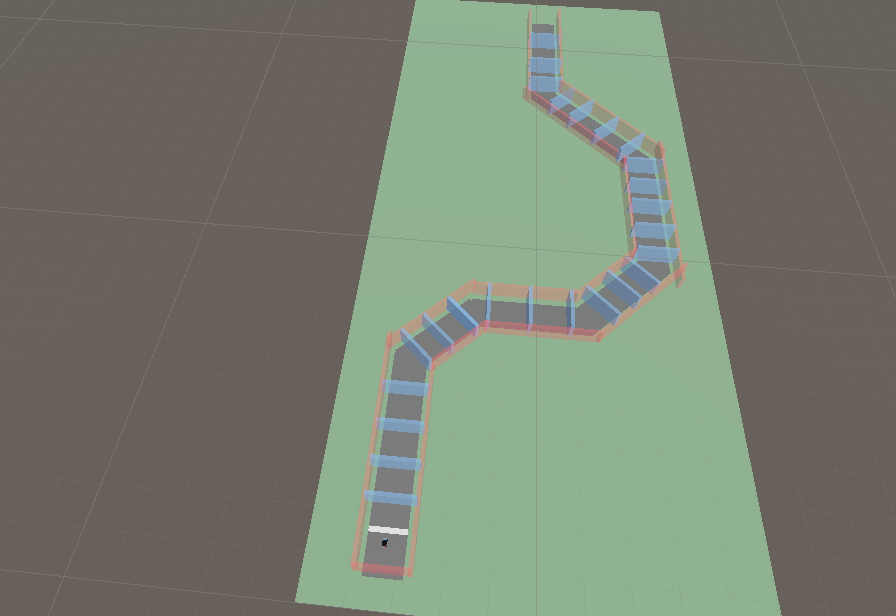
\includegraphics[width=0.6\textwidth]{Images/SprintTrack.png}
\end{center}
\caption{Sprint track}
\label{SprintTrack}
\end{figure}

In the configuration, I set the GAIL and BC to the demonstration I previously created and the training started. The agents were struggling in the first turns, but in short time they got the handle of it and managed to train the track and were successful in finishing it.

To conclude, I think this example was pretty amusing and I got good results. For example, see figure \ref{Sprintracing}, we can see that  the agents are having a pretty close race and they can even throw each other off the track because they all have rigid bodies. The most problematic thing I would say its creating a proper learning environment, because a lot of things can go wrong. It was the main reason of my debugging.

\begin{figure}[h]
\begin{center}
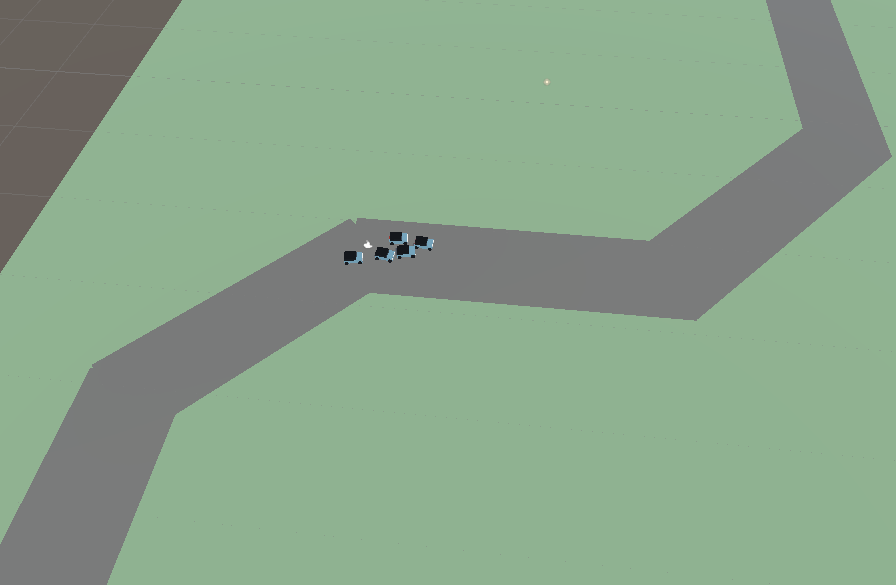
\includegraphics[width=0.6\textwidth]{Images/SprintRacing.png}
\end{center}
\caption{5 agents racing in the sprint track}
\label{Sprintracing}
\end{figure}

\section{Final thoughts}

In conclusion to this chapter, I think the tool can be very useful, but with some limitations. Perhaps if someone wanted to include ML agents in their video game, they would have to figure out a way to train the NPCs. Because, of course, that can not be done in real time, since training takes a lot of computing power and memory. One method that comes to mind is to save the player's play style and later train the NPCs based on those instructions. This has to be done in the background or when the player is offline, so I think there are limited ways you can implement ML-Agents \cite{MLAgents} into your game.

However, I think the technology could work very well for experimentation and indie games. It has acceptable results and I could see it being used, but with previously created models/brains.

\chapter {Conclusion}
\label{ch4}

It can be readily said that current and previous games rely on simpler and more robust techniques. This evolution has led players to grow weary of deterministic and simple AI in games. Just as there is a race for better game graphics, I believe there is also a race for deeper game AI with NNs, BTs, fuzzy logic, genetic algorithms, etc. 

I think the future is taking us step by step to virtual autonomous characters that are lifelike, intelligent, and provide empathy, and I think it's only a matter of time before we can achieve that. I know that so far I have only shown techniques that sell intelligence, not real AI. But I also know that there is significant progress in the techniques shown. If you develop a well-designed game architecture/system and combine it with new AI techniques, the impossible can become possible.

Real game AI is far from complete and unpredictable, perhaps there is no place for it in published video games. But with the curiosity of people experimenting with it, I think the future of real game AI will soon expand to experimentation and indie games.

\cleardoublepage

\printbibliography[heading=bibintoc,type=article,title={Journal articles}]
\printbibliography[heading=bibintoc,type=inproceedings,title={Articles in proceedings}]

\printbibliography[heading=bibintoc,type=incollection,title={Chapters in books}]

\printbibliography[heading=bibintoc,title={Literature}]



\end{document}